\section{Methods and tools}
\label{sec:werkzeuge}

The previous sections described the technologies that directly contributed to the finished application; the following will deal with the tools used for the implementation. This chapter lists all technologies and methods that were used in the development but are not a part of the final product.

To start with, both agile the software development procedure and the test-driven development procedure model are presented. Afterwards, the testing frameworks that helped with the test-driven development will be described. The chapter concludes with a section on development environments.

 
\subsection{Development procedure models}

The procedure model that was chosen is the approach used by agile software development. Test-driven development can be seen as a subset of the procedures own to agile software development. This thesis does, however, rate test-driven development high, which is why an entire section will be devoted to it.

\subsubsection{Agile software development}

Already in the late eighties, the realms of software development echoed growing criticism against conventional phase models and development procedures. \citelit{vorgehen:softwareentwicklung} lists sources of discomfort with the classical life cycle concept. The author does not attribute this discomfort to some sort of vogue; it \enquote{is based on serious experiences with the conventional models and their noticed weaknesses} \citelit[Chap. 2.5.1]{vorgehen:softwareentwicklung}. These include overlong time periods between specification and an executable program, and the insufficient involvement of customers and users; but most notably how strictly successive phases are out of touch with reality.

In 2001, some well-known representatives of agile software development wrote its core values down in the so-called \textit{Agile Manifesto} \cite{agile:manifesto}. These values lay the foundations of the development procedure that is more precisely defined by the manifesto. When applied to the development procedure of the application developed in this thesis, the following goals can be identified:

\begin{itemize}
  \item Frequent feedback and communication between everyone involved in the project
  \item Early and frequent delivery of software; this way, it is possible to verify whether the development procedure is still on the right track to achieve the project's actual goals
  \item The possibility to adjust the initially plans regarding requirements and procedure to the actual requirements
\end{itemize}

Building on the Manifesto's core values, \cite{agile:definition} defines agile software development as follows:

\begin{quote}
Disciplined agile software development is: an iterative and incremental (evolutionary) approach to software development; which is performed in a highly collaborative manner; by self-organizing teams within an effective governance framework; with \enquote{just enough} ceremony; that produces high quality software; in a cost effective and timely manner; which meets the changing needs of its stakeholders. 
\end{quote}

The development in this thesis is done according to the agile methods. This is understood as the established procedure of acting in an agile manner in a part or aspect of the software development \citelit[Chap. 2.4]{vorgehen:agile}. Worth mentioning here are continuous code refactoring, continuous integration and test-driven development.

Code refactoring is defined in \citelit{tdd:unittestframeworks} as \textit{behaviour-preserving transformation}. Accordingly, refactoring is \enquote{the process of transforming source code in order to improve its internal appearance, without changing any functionality} \citelit[p. 2]{tdd:unittestframeworks}. Continuous integration means that all tests are automatically executed when new code is integrated into the project. This process guarantees continued application functionality. Test-driven development is discussed in the next section.


\subsubsection{Test-driven development}
\label{subsec:tdd}

The application is developed in a test-driven manner. Test-Driven Development (TDD) is one of the most important and most widely spread practices in agile software development \citelit[p. 2]{tdd:unittestframeworks}. It was conceived to warrant the quality and serviceability of the program.

\citelit{tdd:unittestframeworks} describes the \textit{test-driven development cycle}. TDD always contains three recurrent steps: \textit{test - code - refactor}.

\begin{description}
  \item[Test] A test for the code to be generated is written and started. Since the code does not yet exist or the desired functionality has not yet been implemented, the test will fail. It is important to proceed in small steps, only testing one aspect of the code at a time.
  \item[Code] The code for the new feature is written in its simplest conceivable implementation. The test will now pass successfully.
  \item[Refactor] The code is now improved by refactoring. Attention should be paid that all the tests must continue to pass successfully.
\end{description}

This method is also called \textit{test-first programming}.

\citelit{tdd:rails} sums up the qualities of a good test. A meaningful test should be \textbf{unambiguous}, i.e. it should produce a discrete yes/no result. Furthermore, it should be \textbf{valid}: the test results have to correspond to the intention of the artifact being tested. A test is \textbf{complete} when it does not need further input to run; a \textbf{repeatable} test is one whose result is deterministic even if the tested system does not behave deterministically. A test should be completely \textbf{isolated}, meaning that the result must not be influenced by results or side-effects of another test. In \citelit{tdd:unittestframeworks}, this anti-pattern is called \textit{test-coupling} which should be avoided. The final trait of a good test requires that tests be able to be started \textbf{automatically}, that they finish in a \textbf{finite} amount of time, and that they may be \textbf{bundled} with other tests into a test suite.

A further development of TDD is \textit{Behaviour-Driven Development (BDD)}. This shifts the stress from the aspect of \enquote{testing} to the aspect of \enquote{prespecification} \citelit[Chap. 1]{bdd}. Similar to domain-driven design, the result is here approximated from the business point of view. In this way, the language with which the problem that needs solving is described can be kept clean of technical terms. There are several BDD frameworks that allow specifications for software to be expressed in executable code:

\begin{quote}
A waterfall \enquote{designer} starts from an understanding of the problem and builds up some kind of model for a solution, which they then pass on to the implementers. An agile developer does exactly the same, but the language they use for the model happens to be executable source code rather than documents or UML. \citelit[Chap. 2]{bdd}
\end{quote}

In practice, the terms TDD and BDD are often used to mean the same thing \cite{bdd:tdd}. In contrast to the misgivings of some developers, TDD/BDD do not usually lead to higher effort and longer development times. The earlier tests exist and the more comprehensive they are, the faster and painless the development cycle becomes. Therefore, the application at hand should be implemented using this method.


\subsection{Testing frameworks}
\label{subsec:testframe}

The tests that were written during the test-driven development can be divided into several layers. \textit{Unit tests} check the functionality of individual software modules. \textit{Integration tests}, on the other hand, verify the interaction between the system's components. Depending on the framework there might be further layers, but it suffices in the scope of this thesis to mention only these two, since they provide a very good functional test coverage when they are combined and well implemented. The following sections will present the particular frameworks.


\subsubsection{JSpec}
\label{subsec:jspec}

A unit test framework is a piece of software that helps writing and executing unit tests. Such frameworks provide a basis that simplifies writing tests, and functionality to perform the tests and output results. Unit tests are developed apart from the actual application; they are not included in the final product. They use the application's objects, but exist only inside the unit test framework. This allows the isolated testing of individual objects without letting them interfere with the actual code \citelit{tdd:unittestframeworks}.

At this point, the limited scope of this thesis allows no substantial comparison of suitable unit test frameworks. An evaluation by the author can be found in \cite{jspec:evaluation}. From many respectable alternatives \cite{jspec:unitlist}, the relatively young framework JSpec was chosen \cite{jspec:website}.

JSpec is similar in functionality and syntax to the BDD framework \textit{RSpec} \cite{rspec:website}, with which Ruby code can be specified and tested. The JSpec syntax is a domain-specific language (DSL) which was specially designed with this purpose in mind.

\textit{Matchers} specify a certain behaviour or the value of an object. \textit{Assertions/expectations} verify this and compare it to a certain value. The keyword {\fontfamily{pcr}\selectfont should} can be compared to the keyword {\fontfamily{pcr}\selectfont assert} from conventional \textit{xUnit test frameworks} that are based on Kent Beck's \textit{SUnit framework}.

\medskip
\begin{lstlisting}[caption=JSpec example: the matcher {\fontfamily{pcr}\selectfont eql}]
{ foo : 'bar' }.should.eql { foo : 'bar' }
\end{lstlisting}

Further examples may be found in the appendix \ref{subsec:testsuite-jspec-code}.

There are also matchers for JQuery functionality that allow the DOM to be tested. JSpec further supports testing asynchronous functions, and provides the option to simulate AJAX requests. Fixtures allow parts of the DOM to be supplied as HTML code.

JSpec can be installed as a Ruby Gem, meaning that tests may be run from the console and integrated into continuous integration. For this purpose it makes use of Rhino \cite{rhino:website}, a Java-based JavaScript interpreter. In the console, it is possible to specify the browser that should be opened in the background; this browser will then execute the tests.

Alternatively, the JSpec library can be included in the JavaScript code. This approach involves opening a HTML file in the browser that will then run the tests. This window will also contain the results. The level of detail and the formatting of the results can be set as parameters in the HTML file. How that looks can be seen in figure \ref{fig:jspec-bad}.

\medskip
\begin{figure}[ht] 
  \begin{center}
    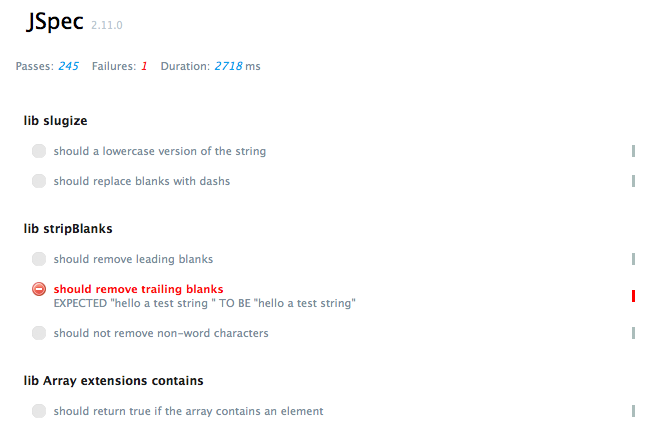
\includegraphics[width=0.9\textwidth]{grafik/jspec-example-bad} 
  \end{center}
  \caption{JSpec: A failing test}
  \label{fig:jspec-bad} 
\end{figure}



\subsubsection{Cucumber}
\label{subsec:cucumber}

With TDD, tests are written before any code is, hence the tests are called black box tests \cite{beck:tdd}. With these, the implementation of the program components that need testing is still unknown: only the expected functionality or rather the result are being tested. For unit tests, this is not always strictly workable, since they meticulously test the components' characteristics. Integration tests, on the other hand, apply at a higher level: a component's functionality is described in a manner that is also understandable for users with no technical background. This allows the developer to think about the business logic without being troubled by implementation details.

Even if a software component has passed a unit test successfully, the quality can only be guaranteed if the component was successfully integrated into the application. The testing framework Cucumber \cite{cucumber:website} provides the tools to create such integration tests.

The test for larger program components that belong together (e.g. user administration, usage of the outliner) is called a \textit{feature} in Cucumber's \textit{Domain Specific Language (DSL)}. Every feature specifies the role of the user (\textit{As a}), the content of the feature (\textit{I want}), and a goodwill (\textit{In order to}). A feature contains several \textit{stories} that each describe the execution of a software function from the beginning to the end (e.g. user log-in, indent a line). A story contains the preconditions (\textit{Given}), the individual steps a user makes (\textit{When}) and the expected results (\textit{Then}). An example from the project can be found in listing \ref{lst:cucumber-feature}.

\lstset{language=ruby, style=cucumber}
\medskip
\begin{lstlisting}[caption=A Cucumber feature with two scenarios,label=lst:cucumber-feature]
Feature: CRUD for outlines
  In order to sort my notes
  As a user
  I want to create, list, update and delete outlines
  
  Scenario: create an outline with note
    When I go to the start page
      And I follow "New Outline"
      And I fill in "title" with "Songs"
      And I press "Save"
    Then I should see "Songs"
      And I should see "Here is your new outline"
      And the new note li should be blank
      
  Scenario: edit an outlines title
    Given an outline with the title "Songs"
      And I save
    When I go to the start page
      And I follow "Songs"
      And I follow "Change title or delete this outline"
      And I fill in "title" with "Tunes"
      And I press "Save"
    Then I should see "Title successfully changed"
      When I go to the start page
    Then I should see "Tunes"
      And I should not see "Songs"
\end{lstlisting}

The meaning of individual rows, called \textit{steps}, has to be defined in further files. Every step consists of a signal word and a regular expression for which a block of ruby code is executed. In the process, the results of the matching groups are fed to the block as a regular expression. This is exemplified in listing \ref{lst:cucumber-steps}.

A feature can be executed from the command line (for example in figure \ref{fig:cucumber-bad}). The successful steps are printed in green; the ones that failed are printed in red including their error messages.

\medskip
\begin{lstlisting}[caption=Cucumber step definition,label=lst:cucumber-steps]
Given /^an outline with the title "([^\"]*)"$/ do |title|
  outline = {:kind => 'Outline', :title => title}
  RestClient.put "#{host}/#{database}/#{title}", outline.to_json
end

When /I fill in "(.*)" with "(.*)"/ do |field, value|
  find_by_label_or_id(:text_field, field).set value
end
\end{lstlisting}

\medskip
\begin{figure}[ht] 
  \begin{center}
    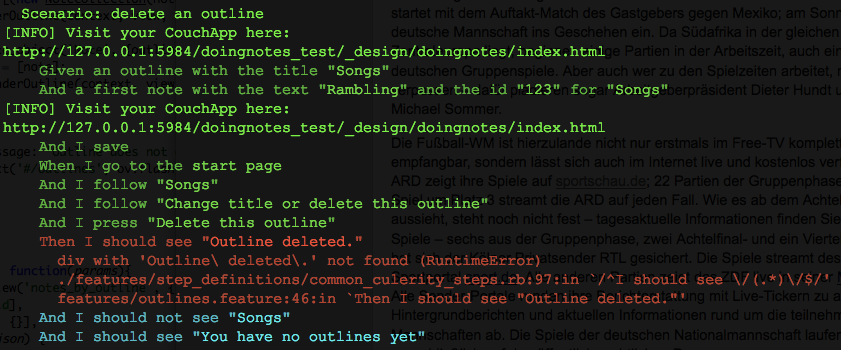
\includegraphics[width=\textwidth]{grafik/cucumber-example-bad} 
  \end{center}
  \caption{Cucumber: A failing test}
  \label{fig:cucumber-bad} 
\end{figure}




\subsection{Development environments}

\subsubsection{Textmate}

TextMate \cite{textmate:website} is a text editor for the operating system Mac OS X. Textmate was released in 2004 by Alan Odgaard. In August 2006, the program was awarded the \enquote{Apple Design Award for Best Developer Tool} at Apple's \enquote{Worldwide Developers Conference}. TextMate is a very clearly-arranged editor \citelit{textmate:latex}. It does not boast the same functional range as Eclipse or NetBeans, but its functionality can be expanded at will thanks to its broad support for scripts and plug-ins. For the development of the task at hand, an integrated development environment wouldn't be helpful: the specific requirements for developing a CouchApp are currently not met by Eclipse.

Textmate provides syntax highlighting for all the languages used, auto-completion inside a file, project-wide searching, easy access to all files in a project, an easy-to-use interface with tabs for all open files. In addition, it is easy to adjust Textmate to particular needs. For example, a special CouchApp macro was written to update the design documents in the database, something that accelerated the development process.

\subsubsection{Firefox / Firebug}

Section \ref{subsec:nochanges} explains why the web browser Firefox \cite{firefox} in version 3.6 or higher was chosen as the target platform. Because of this, the application was developed with the aid of the firefox add-on Firebug \cite{firebug}.

Firebug allows developers to examine style sheets, HTML, the DOM and JavaScript on a page. A console allows logging HTTP requests and log statements in the JavaScript code. The source code of a website can also be analysed and edited on-the-fly. This makes debugging easy. The tool is therefore extremely popular amongst web developers \cite{firebug:beliebt}. Firebug is the sixth most downloaded add-on for Firefox \cite{firebug:haeufig}. It is used on a daily basis by two million people \cite{firebug:stats}.

In this project, Firebug was used for the development of the DOM, for the shaping of the front-end, and for the optimisation of the site's performance.